%----------------%
\chapter{Results}
%----------------%

Our implementation lays the foundation for the \pfs language server and verifies
the feasibility of the design decisions made in chapter~\ref{ch:design}. We have
implemented the \acrshort{p4} Analyzer pipeline, which consists of the lexer,
the preprocessor, a generic parser library, and a proof-of-concept grammar for
\acrshort{p4}\textsubscript{16}. \acrshort{p4} Analyzer integrates tightly with
Visual Studio Code and other \acrshort{lsp} clients, providing autocompletion,
diagnostics, and limited go-to-definition functionality. The server is resilient
to common errors in user input. The project's integration with VS Code ensures
that the core analyzer is restarted if it encounters fatal errors.

%-----------------------------------------%
\section{Overview of implemented features}
%-----------------------------------------%

\begin{figure}[h]
	\centering
	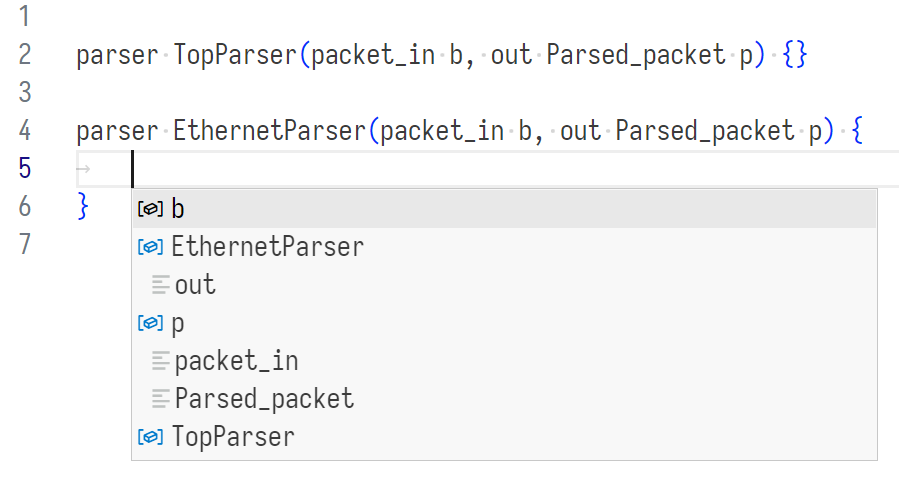
\includegraphics[width=\textwidth]{resources/p4analyzer-autocompletion.png}
	\caption{Autocompletion in Visual Studio Code. The blue items are suggested
	from definitions recognised by the parser, while grey items are simply
	identifiers in the preprocessed token stream.}
	\label{fig:autocompletion}
\end{figure}

The lexer and preprocessor parts of the pipeline have been implemented quite
thoroughly, with good error recovery and feature sets on par with the design
presented in chapter~\ref{ch:design}. Lexer and preprocessor error channels
propagate to the \acrshort{lsp} client with understandable error messages. The
preprocessor, in particular, attempts to recover from missing or superfluous
directives, and suggests possible fixes to the user. It also detects circular
file inclusion problems.

One feature that is currently lacking is the precise tracking of source
locations via the ``inclusion path'' mechanism. This requires some changes in
the preprocessor, but not a significant refactor. One more concern is the
evaluation of complex conditions for conditional inclusion directives. If the
condition contains references to macros outside the \texttt{defined} construct,
these macros could, depending on their definition, change the syntactic meaning
of the condition, and therefore influence evaluation. A simple fix for this
issue is to store conditions as strings and parse them on-demand after
performing macro expansion, at the expense of some computational overhead.
However, such use cases are rare, so this is not considered a priority for the
project.

The parser, on the other hand, is only a proof-of-concept. While the test suite
indicates that the library handles edits correctly, integrating this custom
approach to incrementality with the Salsa library is not straightforward.
Currently, the parser reparses preprocessed token streams from scratch. Parsing
is still memoized as a Salsa query, so it happens on-demand and only after
edits. Error labels, discussed in the parser design section, have not been
implemented yet, and the parser still reports at most one error to the user.

While we deem the \acrlong{ast} \acrshort{api} rather robust, owning to its
success in the rust-analyzer project, its scope and usefulness hinges on a
well-designed grammar for the \pfs language. The current grammar is very lacking
in this regard. The go-to definition functionality relies on the semantic
\texttt{definition} non-terminal and its correct use in the grammar. Currently,
it does not respect lexical scoping -- the grammar requires a larger overhaul,
possibly supported by extensions to the supported \acrshort{peg} constructs, in
order to meaningfully recognise scoped syntactic constructs.

\begin{figure}[t]
	\centering
	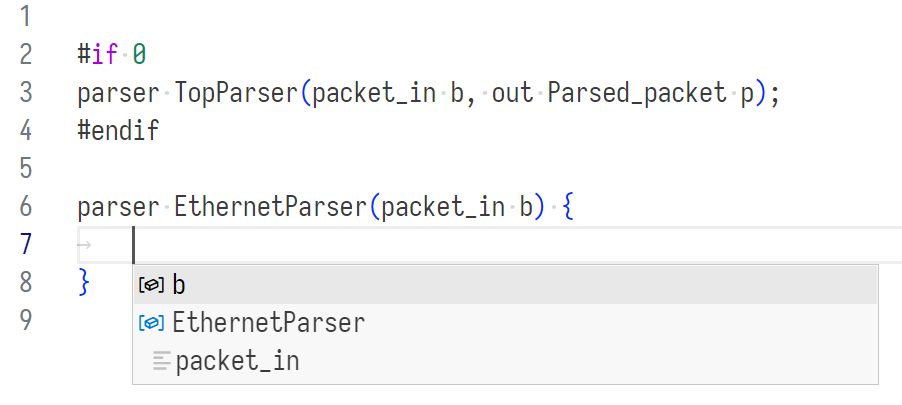
\includegraphics[width=\textwidth]{resources/p4analyzer-preprocessor-response.png}
	\caption{The set of suggested identifiers depends on preprocessor
	directives.}
	\label{fig:preprocessor-response}
\end{figure}

\begin{figure}[t]
	\centering
	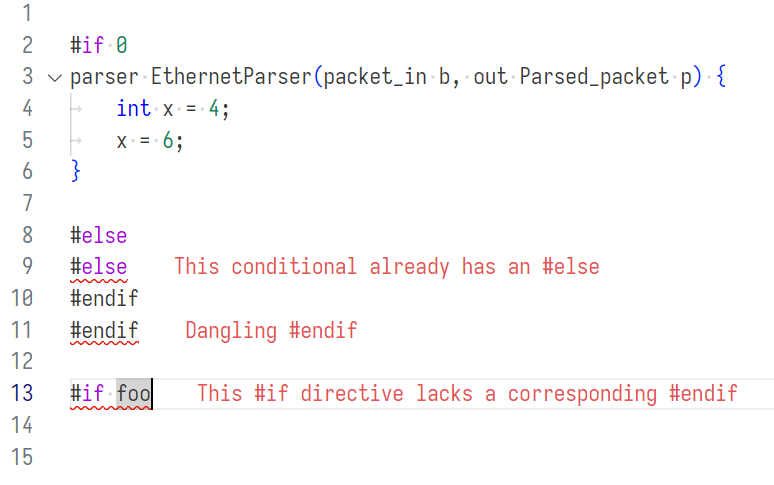
\includegraphics[width=\textwidth]{resources/p4analyzer-preprocessor-errors.png}
	\caption{The preprocessor continues to produce output even in the presence
	of several errors.}
	\label{fig:preprocessor-errors}
\end{figure}


\begin{figure}[t]
	\centering
	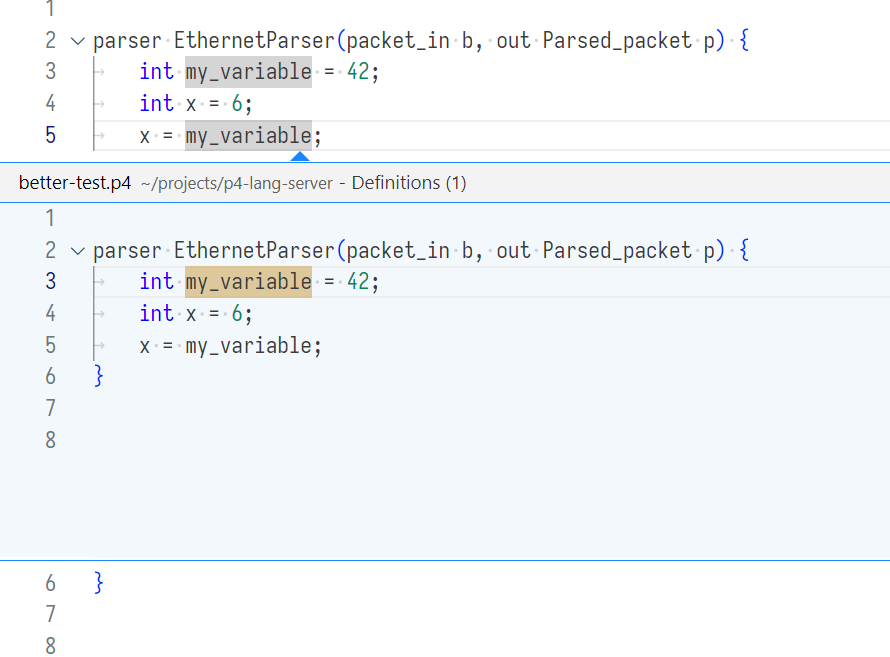
\includegraphics[width=\textwidth]{resources/p4analyzer-goto-definition.png}
	\caption{Rudimentary support for go-to definition is also available.}
	\label{fig:goto-def}
\end{figure}

%---------------------%
\section{Benchmarking}
%---------------------%

An important consideration for an interactive developer tool is its performance.
Our test suite includes lexer and parser throughput measurements in the form of
micro-benchmarks based on the \texttt{criterion}
library\footnote{\url{https://crates.io/crates/criterion}}.

\begin{table}[h]
	\centering
	\begin{tabular}{lrrr}
		\hline
		\textbf{Benchmark}         & Min       & \textbf{Mean} & Max \\
		\hline
		\texttt{lexer baseline}    & 4.95   ms & 5.00   ms & 5.06   ms \\
		\texttt{lexer timing}      & 130.46 ms & 132.41 ms & 134.61 ms \\
		\texttt{parser baseline}   & 0.31   ms & 0.31   ms & 0.31   ms \\
		\texttt{parser timing}     & 187.33 ms & 189.38 ms & 191.63 ms \\
		\hline
	\end{tabular}
	\caption{Lexer and parser timings, statistics of 100 samples.}
	\label{tab:throughput}
\end{table}

Table~\ref{tab:throughput} shows the results of the throughput benchmarks. Some
context is necessary to understand these measurements.

\begin{description}
	\item[Lexer baseline] This benchmark measures only the overhead of copying
		the input and converting it from a UTF-8 string into a vector of
		individual codepoints. It does not involve the lexer at all.
	\item[Lexer timing] This benchmark runs our lexer on example \pfs code
		adapted from the specification\cite{p416:v123:spec}. This is roughly
		\(200\) lines of code, concatenated with itself \(1,000\) times. The
		total measurement is the time it takes to lex this input (\(200,000\)
		lines, about \(4.8\) megabytes when packed as UTF-8).
	\item[Parser baseline] The parser baseline measures the overhead of
		constructing a parser and initializing it with input. It is measured on
		the same input string and grammar as the \textbf{parser timing}
		benchmark. It copies the input string into a vector (similarly to the
		lexer baseline), then back into a UTF-8 string. This benchmark does not
		invoke the parser.
	\item[Parser timing] This benchmark measures the time it takes to parse a
		long arithmetic expression in a simple grammar, shown in
		Listing~\ref{lst:parser-benchmark-grammar}. The expression is a randomly
		generated sequence of integers, with addition and subtraction operations
		interspersed throughout. The input string has only \(100,000\)
		characters. Note that input generation is not a part of the benchmark
		and that the benchmark harness verifies that the expression parses
		correctly before initiating the measurement.
\end{description}

As the measurements show, the lexer is fast with throughput well over one
million lines of \acrshort{p4}, or over \(30\) megabytes per second. The parser
is significantly slower: when operating on character tokens (Unicode code
points), it can only parse roughly \(0.5\) megabytes per
second\footnote{Assuming a packed representation, to relate to the given lexer
measurements, even though, in this case, the parser works with a vector of
4-byte characters instead.}.

\begin{lstlisting}[
	caption={The grammar used in the parser benchmark.},
	label={lst:parser-benchmark-grammar},
	language=Rust,
	tabsize=4,
	float,
]
let grammar = grammar! {
	start => num, expr_chain;
	expr_chain => expr_choice rep;
	expr_choice => add_chain | sub_chain;
	add_chain => plus, num;
	sub_chain => minus, num;
	plus => "+";
	minus => "-";
	num => digit, many_digits;
	many_digits => digit rep;
	digit => n0 | n1 | n2 | n3 | n4 | n5 | n6 | n7 | n8 | n9;
	n0 => "0";
	n1 => "1";
	// etc.
};
\end{lstlisting}

%--------------------------------%
\section{The open-source project}
%--------------------------------%

\acrshort{p4} Analyzer was open-sourced on April 18, 2023. The project is
available on GitHub under the umbrella of the \acrshort{p4} language
organization\footnote{\url{https://github.com/p4lang/p4analyzer}}. It is
permissively licensed under the terms of the Apache 2.0 license. Despite its
fairly quiet release, it gathered significant attention both internally within
Intel and from the \acrshort{p4} community.

We have discovered that in 2023, a research group at McMaster University has
independently started a very similar project. Their \pfs language server is also
developed in Rust and is available from the ACE Design organization's
GitHub\footnote{\url{https://github.com/ace-design/p4-lsp}}. We have since
gotten in touch with the researchers working on it and are looking for ways to
collaborate.

%--------------------%
\section{Future work}
%--------------------%

As is clear from our results so far, there is much more work left to be done.
After finalising the parser, future development efforts should aim to cover more
of the \acrshort{api} surface of \acrshort{lsp} and provide useful features. In
particular, we would like to develop lints\footnote{Soft warnings about code
style and possible bugs.} and code navigation features built on the
\acrshort{ast} abstraction framework. Rust makes usage of iterators ergonomic
and efficient. We remain optimistic that the architecture of \acrshort{p4}
Analyzer presented in this thesis will serve future extensions well.
